\documentclass{standalone}
\usepackage{tikz}
\usetikzlibrary{shapes}
\usetikzlibrary{positioning}
\usepackage{amsmath}


%\tikzstyle{startstop} = [rectangle, rounded corners, text width=2cm,text centered, minimum height=1cm, draw=black]
% \tikzstyle{io} = [trapezium, trapezium left angle=70,trapezium right angle=110, text width=3.5cm, minimum height=1cm, text centered, draw=black, trapezium stretches=true]
% \tikzstyle{process} = [rectangle, text width=3.5cm, minimum height=1cm, text centered, draw=black]

\begin{document}
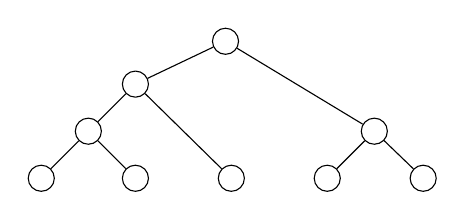
\begin{tikzpicture}[node distance=2cm]

    % \node(start)[startstop]{Start};
    
    \node(B)[draw, circle, minimum size=0.2cm]{};
    \node(A)[draw, circle, minimum size=0.2cm, above right=0.3cm and 0.9cm of B]{};
    \node(D)[draw, circle, minimum size=0.2cm, below left=0.5cm of B]{};
    \node(F)[draw, circle, minimum size=0.2cm, below left=0.5cm of D]{};
    \node(G)[draw, circle, minimum size=0.2cm, below right=0.5cm of D]{};
    

    \node(E)[draw, circle, minimum size=0.2cm, right=0.8727922cm of G]{};
    \node(C)[draw, circle, minimum size=0.2cm, right=0.8727922cm of E]{};
    \node(I)[draw, circle, minimum size=0.2cm, above right=0.5cm of C]{};
    \node(H)[draw, circle, minimum size=0.2cm, right=0.8727922cm of C]{};

    \draw (A) -- (B) -- (D) -- (F);
    \draw (D) -- (G);
    \draw (B) -- (E);
    \draw (A) -- (I);
    \draw (I) -- (C);
    \draw (H) -- (I);
    



    % \node(train1)[process, above right = 1cm and 0.75cm of rollingorigin, ]{Obtain $h$-step-ahead forecasts for each window};
    % \draw[->] (rollingorigin.north) |- (train1.west) ;
    % \node(train2)[process, right of=rollingorigin]{Obtain $h$-step-ahead realization for each window};
    % \draw[->] (rollingorigin.east) -- (train2.west) ;
    % \node(train3)[process, right of=train2]{Train reconciliation matrix $A_1,\dots,A_h$};
    % \draw[->] (train2.east) -- (train3.west);
    % \draw[->] (train1.east) -| (train3.north);

    % \node(forecast1)[process,below right = 1cm and 0.75cm of rollingorigin]{Obtain $h$-step-ahead base forecasts $\hat{\mathbf{\pi}}_{T+1},\dots,\hat{\mathbf{\pi}}_{T+h}$};
    % \draw[->] (rollingorigin.south) |- (forecast1) ;
    % \node(forecast2)[process, right of=forecast1]{Obtain $h$-step-ahead reconciled distribution};
    % \draw[->] (forecast1) -- (forecast2);
    % \node(output)[io, right of=forecast2]{Output coherent forecast $\tilde{\mathbf{\pi}}_{T+1},\dots,\tilde{\mathbf{\pi}}_{T+h}$};
    % % % \node(end)[startstop, below of=output]{End};

    % % % \draw[->] (start) edge (in)
    % % 
    % % 

    % % \draw[->] (train1) |- (train3);
    % %\draw[->] (in.east) -| (forecast1.north);
    % \draw[->] (train3.south) -- (forecast2.north);
    % \draw[->] (forecast2) -- (output);
    % % 


    % % \draw[->] (forecast2) -- (output);
    % % \draw[->] (output) -- (end);

\end{tikzpicture}
\end{document}
